%卒論概要テンプレート ver. 4.0

\documentclass[uplatex,twocolumn,dvipdfmx]{jsarticle}
\usepackage[top=22mm,bottom=22mm,left=22mm,right=22mm]{geometry}
\setlength{\columnsep}{11mm}
\usepackage[T1]{fontenc}
\usepackage{txfonts}
\usepackage[expert,deluxe]{otf}
\usepackage[dvipdfmx,hiresbb]{graphicx}
\usepackage[dvipdfmx]{hyperref}
\usepackage{pxjahyper}
\usepackage{secdot}





%タイトルと学生番号,名前だけ編集すること
\title{\vspace{-5mm}\fontsize{14pt}{0pt}\selectfont 文書自動添削システムによる学生の文書改善履歴の調査}
\author{\normalsize プロジェクトマネジメントコース 矢吹研究室 1442031 氏名 小山隆太郎}
\date{}
\pagestyle{empty}
\begin{document}
\fontsize{10.5pt}{\baselineskip}\selectfont
\maketitle





%以下が本文
\section{序論}
学生が行う研究では,研究だけではなく文書を作成する時間が長い.卒業論文は文量が多く,執筆形式も指摘される.大量の文書を人の目で添削を行うことには限界があり,かかる労力は大きい.

そこで,継続的インテグレーション\cite{a}を用いることで,文書添削を自動化できないか考えた.継続的インテグレーションとは,プログラムのビルドやテスト等を継続的に実行していくことである.

また,自分以外が読んでもわかりやすい文書を書く必要があり,文が長いほど理解が難しくなってしまう場合や,口語が混じり,文書の質が落ちてしまうことがある.

このような状況に文書自動添削ツールであるRedPenを活用することで,文書の質が向上すると考えた.継続的インテグレーションとRedPenを組み合わせ,文書添削を自動化するツールを構築する.

\section{目的}
文書添削の機能を確立することが目的である.RedPenには,複数の添削機能を提供するほか,添削機能を新たに作成することが可能である.既存の添削機能と作成した添削機能を組み合わせ,添削機能の質を高める.

\section{手法}
\begin{enumerate}
\item 添削機能を作成し,GitHubに文書をアップロードすると,文書チェックプログラムが自動で動作するようにし,文中のミスを出力する. 
\item 添削結果を記録し,文中のミスが減るか推移を得る.
\end{enumerate}

\section{結果}
矢吹研究室に所属する3年生が書いた課題研究の概要文の添削を行った際の,エラー数の推移は図\ref{conf}のとおりである.各折れ線が文章1つのエラー数の推移を表している.エラー数が減った文書の修正は以下のように行われた.

\begin{enumerate}
\item 「の」,「が」等の接続詞の多用や,同一単語の複数回利用を抑えたことで,文長を短くした.「丁度」,「ちょうど」といった同じ言葉の表記を統一し,数値の全角表記を半角に修正した. 
\item 「これ」,「あれら」等の指示語の利用を抑えた文書.「感じる」,「思う」といった感嘆符の利用を避け,断定系に修正した文書は右下がりの推移を得た.
\end{enumerate}

\begin{figure}[htb]
\centering
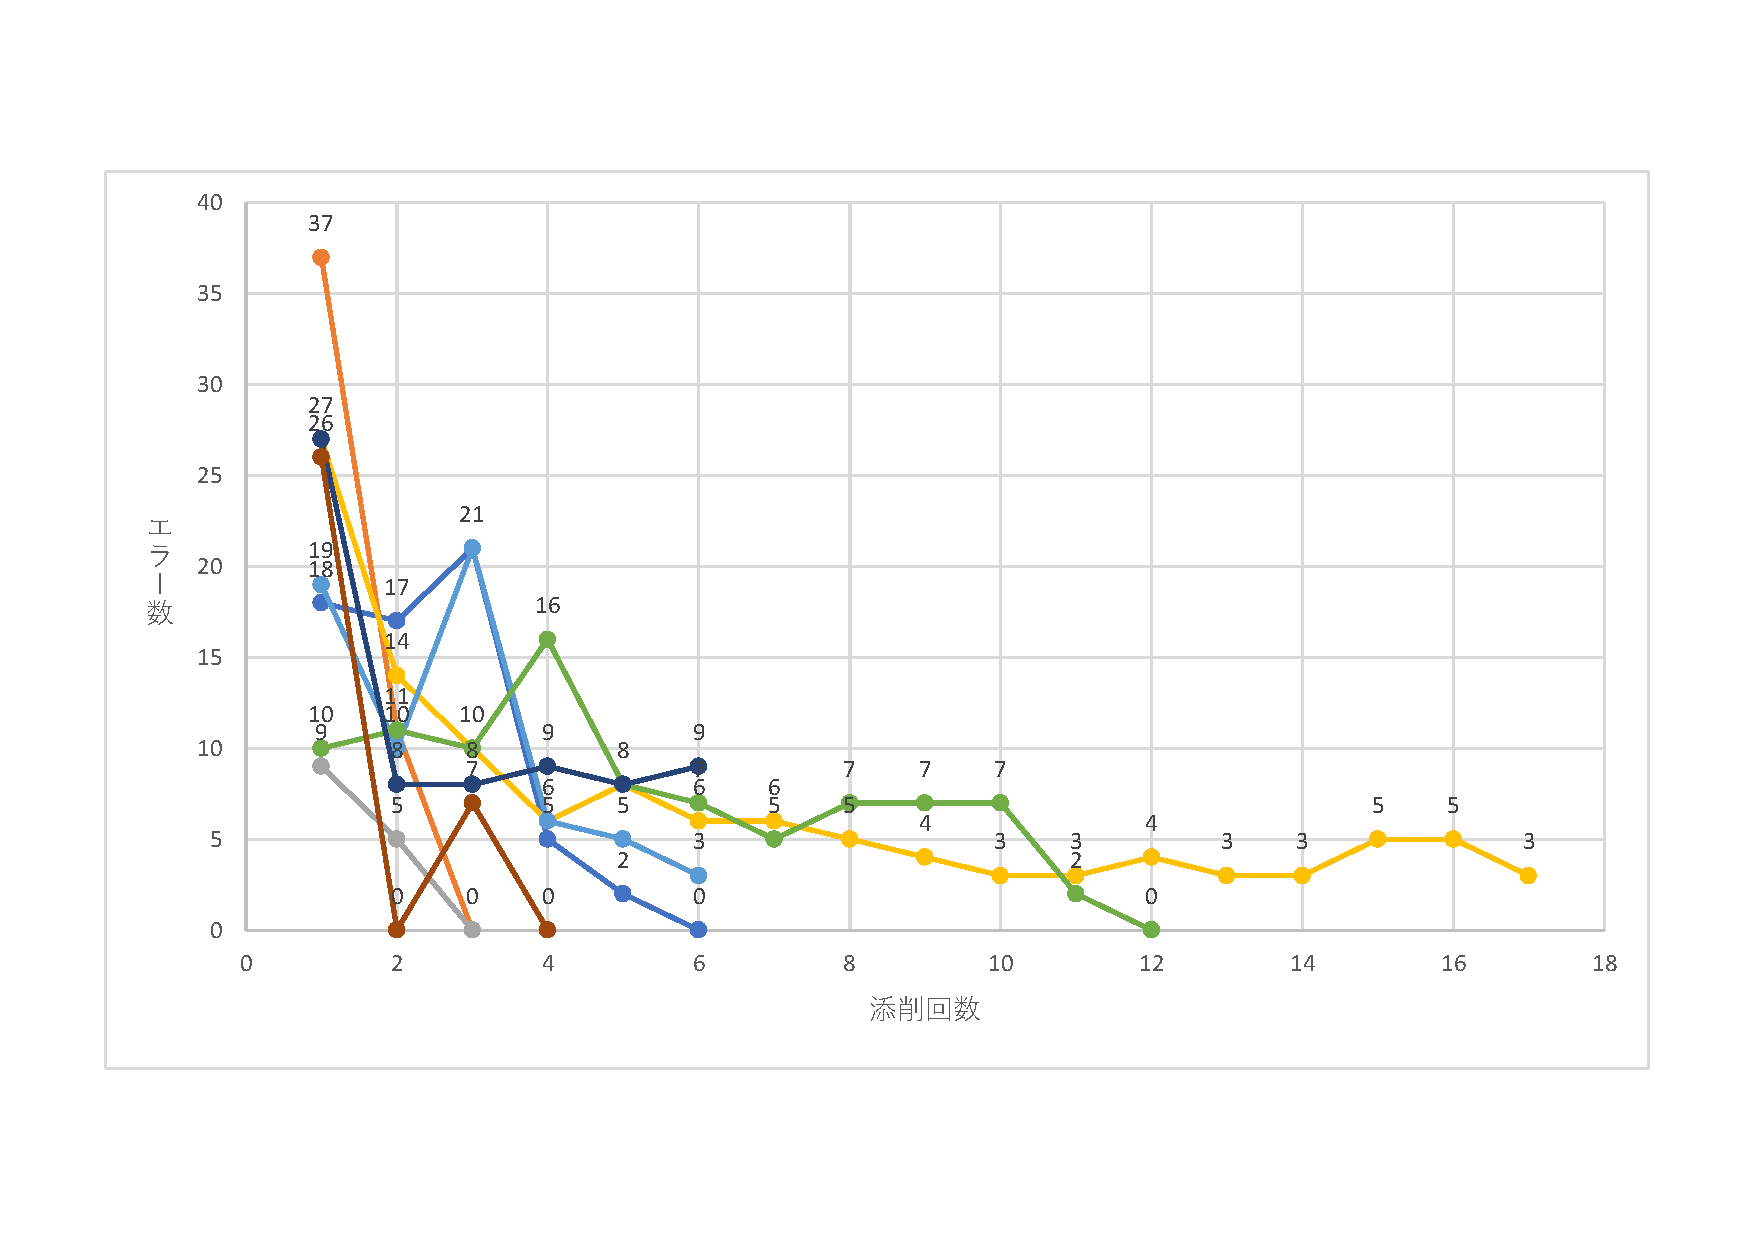
\includegraphics[width=6cm,clip]{redpen.pdf}
\caption{添削マシンを使用した文書の添削項数の推移}\label{conf}
\end{figure}

\section{考察}
指示語の利用を避けるルールと,断定系を使用するよう指示するルール等を作成したところ,専門用語を用いて解説する文書を多く見ることができた.「感じる」,「考えられる」等の利用を避け,「考える」,である調を使用し解説したことで,結論に安心感を与える文書を作成することができた.

\section{結論}
RedPenに新しい添削機能を作成し,文書添削をしたことで,文書校正や形式の文中ミスの削減ができた.添削マシンを利用した際の文書作成時間に変化について,今後検証が必要である.





\bibliographystyle{junsrt}
\bibliography{biblio}%「biblio.bib」というファイルが必要.

\end{document}
